%\documentclass[11pt, a4paper, useAMS,usenatbib]{mn2e}
%\documentclass[usenatbib]{mn2e}
\documentclass[useAMS,usenatbib]{mn2e}

%define general packages
%\usepackage{epsfig}
\usepackage{amsmath}
%\usepackage{natbib}
%\usepackage{epstopdf}

\usepackage{epsfig}
\usepackage{epstopdf}
\usepackage{lscape} % Allows landscape environment to be used
\usepackage{natbib}
\usepackage{tabularx}
\usepackage{multirow}
\usepackage{amssymb}
\usepackage{gensymb}

\def\gtrsim{\mathrel{\hbox{\rlap{\hbox{\lower4pt\hbox{$\sim$}}}\hbox{$>$}}}}


\title{FRB repetition and non-Poissonian statistics}
\author[Connor et al.]{
Liam Connor$^{1,2,3}$\thanks{E-mail:\ connor@astro.utoronto.ca}
Ue-Li Pen$^{1, 6, 7}$\thanks{E-mail:\ pen@cita.utoronto.ca}
Niels Oppermann$^{1}$\thanks{E-mail:\ niels@cita.utoronto.ca}
\\
$^1$ Canadian Institute for Theoretical Astrophysics, University of Toronto, M5S 3H8 Ontario, Canada
\\
$^2$ Department of Astronomy and Astrophysics, University of Toronto, 
M5S 3H8 Ontario, Canada
\\
$^3$ Dunlap Institute for Astronomy and Astrophysics, University of Toronto,
Toronto, ON M5S 3H4, Canada
\\
$^6$ Canadian Institute for Advanced Research, Program in Cosmology
and Gravitation
\\
$^7$ Perimeter Institute for Theoretical Physics, 31 Caroline St. N., Waterloo, ON, N2L 2Y5, Canada
}


\begin{document}
\date{\today}
\pagerange{\pageref{firstpage}--\pageref{lastpage}} 
\pubyear{2015}
\maketitle
\label{firstpage}

\begin{abstract}
We discuss some of the claims that have been made regarding the statistics of 
fast radio bursts (FRBs). In \cite{2015arXiv150505535C} we conjectured that flicker noise associated 
with FRB repetition could show up in non-cataclysmic neutron star emission models,
like supergiant pulses. We show how if their repeat rate really were non-Poissonian
and had a pink or red spectrum then the current limits of repetition ($\lesssim$ daily)
would be weakened. The repeat rate has implications for observing strategy, generally favouring 
shallow wide-field surveys, including if it is zero. 
We also discuss the statistics of the apparent latitudinal dependence of FRBs, and offer
a simple method for calculating the significance of this effect. It is shown how 
the evidence for a steep latitudinal gradient is less strong than initially suggested 
and simple explanations like increased scattering and sky temperature 
in the plane are sufficient to decrease the low-lat burst rate, given current data.
The reported dearth of bursts near the plane is further complicated if FRBs have 
non-Poissonian repetition, since in that case the effective event rate itself 
depends on survey depth.

\end{abstract}
\begin{keywords}
\end{keywords}

\newcommand{\be}{\begin{eqnarray}}
\newcommand{\ee}{\end{eqnarray}}
\newcommand{\beq}{\begin{equation}}
\newcommand{\eeq}{\end{equation}}

\section{Introduction}
There is mounting evidence that the new class of transients 
known as fast radio bursts (FRBs) are of astronomical origin.
The most striking features of FRBs are their large dispersion
measures (DMs) -- too high to be attributed to our own Galaxy's
ISM --
and their event rate (10$^3-10^4$ sky$^{-1}$ day$^{-1}$). They
last for $\sim$millisecond with peak flux of $\sim$Jy, and none
has been conclusively shown to repeat. This has lead to the 
interpretation that FRBs are cosmological,
since the intergalactic medium (IGM) would naturally provide
DMs between $\sim$300-1600 pc cm$^{-3}$ for sources at 
$z\sim0.3-1$ \citep{2013Sci...341...53T}. 

Given their apparent phenomenological richness
(polarization, scattering, etc.) and considering
how little we know about their location and physical 
origin, it is likely that FRBs will be of interest to the community for 
years to come, assuming they are not terrestrial.
Though we are in the regime of only $\sim$dozen published FRBs, 
at present the conventional wisdom is that they are likely cosmological
in origin \citep{2013Sci...341...53T}, they seem to not repeat regularly
\citep{2015MNRAS.454..457P}, and there is a dearth of bursts 
at low Galactic latitudes \citep{2014ApJ...789L..26P, 2014ApJ...792...19B, 2015MNRAS.451.3278M}.

Based on this premise there have been 
a number of models proposed to describe cataclysmic, cosmological 
FRBs \citep{2012ApJ...760...64M, 2013PASJ...65L..12T, 2014A&A...562A.137F, 2015ApJ...814L..20M}.
However since the field is still in its infancy it is important to
leave as many conceptual doors open as possible;
assumptions about the statistics of their event rate, 
spatial distribution, and repetition are important for the design
and observing strategy of upcoming surveys. In section \ref{repeat} we explore the 
consequences of repeating FRBs in the case where their 
burst rate is non-Possionian and exhibits a 1/$f$ power spectrum, 
or pink noise. We also investigate the claims of \cite{2015arXiv150701002M}
that FRB 140514 could have been the same source as FRB 100220, 
and comment on its implications. In section \ref{rate}
discuss the impact of FRB repetition on survey strategy. In section \ref{latitude}
we discuss the statistical treatment of the apparent latitudinal dependence 
of event rate and the lack of detections at low Galactic latitude.

% Usual FRB introduction, swayed towards repetition and statistics.

\section{Repeat rates}
\label{repeat}

Though no source has been shown with certainty to repeat, 
the limits on the repeatability of FRBs are still weak. Several 
models generically predict repetition, whether periodic or stochastic. 
Galactic flaring stars \citep{2015arXiv150701002M}, radio bursting 
magnetars \citep{2007arXiv0710.2006P, 2015ApJ...807..179P}, and pulsar planet systems 
\citep{2014A&A...569A..86M} all predict repetition with varying 
rates and burst distributions. 

In \cite{2015arXiv150505535C} we 
suggest supergiant pulses from very young pulsars in supernova 
remnants of nearby galaxies could explain the high DMs, Faraday rotation, 
scintillation, and polarization properties of the observed FRBs. We  
proposed that if the repetition of supergiant pulses were non-Poissonian 
(with a pink or red distribution) 
then one might expect several bursts in a short period of time. 
It is also worth mentioning that the statistics and repeat rates of FRBs 
could vary from source to source -- even if 
they come from a single class of progenitors -- so a long follow-up on an individual burst 
may not provide global constraints.
In this 
letter we will refer to stationary Poisson processes ($\mu(t)$ is constant)
as ``Poissonian". When we discuss non-Poissonian statistics we will be
focusing on stochastic processes that are correlated on varying timescales. For
example we will not discuss periodic signals, which are not Poissonian but 
we feel they have already been studied \citep{2015MNRAS.454..457P}.


\subsection{Flicker noise}

Pink noise is ubiquitous in physical systems, showing up in 
geology and meteorology, a number 
of astrophysical sources including quasars and the sun, 
human biology, nearly all electronic devices, finance, 
and even music and speech
\citep{1978ComAp...7..103P, 1975Natur.258..317V}.
Though there is no agreed upon
mathematical explanation for this phenomenon
 \citep{2002physics...4033M}, fluctuations 
are empirically known to be inversely proportional to frequency 
for a variety of dynamical systems. This can be written as 

\begin{equation}
S(f) = \frac{C}{f^\gamma} \,\,\,\,\,\ \textup{if} \,\,\,\,\, f_{min} \le f \le f_{max}
\end{equation}

\noindent where $S(f)$ is the spectral density (i.e. powerspectrum), $\gamma$ is 
between 0.5-2,
and $f_{min}$ and $f_{max}$ are cutoffs beyond which the powerlaw 
does not hold.

In the case of a time-domain astronomical 
source, this results in uniformity on short timescales, i.e. a burst of 
clustered events followed by extended periods of quiescence. 
If FRBs were to exhibit such flicker noise then their repetition would 
not only be non-periodic, but would also have a time-varying 
pulse rate. Therefore the number of events
seen in a follow-up observation would depend strongly on 
the time passed since the initial event.

In \cite{2015MNRAS.454..457P}
the fields of eight FRBs discovered between 2009 and 2013
were followed up from April to October of 2014, for an average 
of $\sim$11.4 hours per field. During this follow-up programme 
FRB 140514 was found in the same beam as FRB 110220, however
the authors argue that it is likely a new source due to its lower DM. 
After its discovery, the field of 140514 was monitored 
five more times, starting 41 days later on 2014-05-24, without seeing anything.
Under the assumption that 140514 was a new FRB 
that only showed up in the same field 
coincidentally and that the repeat rate is uncorrelated,
 \cite{2015MNRAS.454..457P} rule out repetition with P $\le$ 8.6 
hours and reject 8.6 $<$ P $<$ 21 hours with 90$\%$ confidence.
However it is possible that one or both of those premises 
is invalid, so it is useful to explore the possibility of non-stationary 
repeat rate statistics and repeating FRBs with variable DM. 

If the statistics of the FRB's repeat rate were
non-Poissonian and initial bursts from FRBs were to have aftershocks
similar to earthquakes, then the non-immediate follow-up observations 
impose far weaker repeat rate limits than has been suggested. We 
constructed a mock follow-up observation of the eight FRBs whose
fields were observed in \cite{2015MNRAS.454..457P}. We then 
asked how many bursts are seen to repeat if we do an immediate
follow up vs. a follow-up several years after the initial event 
at times corresponding to 
to the actual observations carried out. 

We Monte Carlo this 
simple simulation with one sample per hour and a probability of 0.5 
that a given sample has a burst in it. The repeat rate of once per two hours
is chosen arbitrarily and should not affect the comparison. 
In the stationary Poisson case, the rate of bursts in 
the immediate follow-up is the same as the multi-year follow-up 
since all times are 
uncorrelated. However with flicker noise 
the variance is strongly time dependent. If we imagine an object that 
repeated on average once per hour, then if those pulses were Poisson-distributed 
the probability of seeing zero bursts in 10 hours or longer is $\sim$0.01. With 
pink noise one expects this roughly 20$\%$ of the time, since the system 
prefers either to be in ``on" or ``off" mode. If the average repeat period were more 
like 5-20 hours, then we would often see nothing in a multi-day follow-up 
observation that took place weeks or years after the initial event.


\begin{figure}
  \centering
   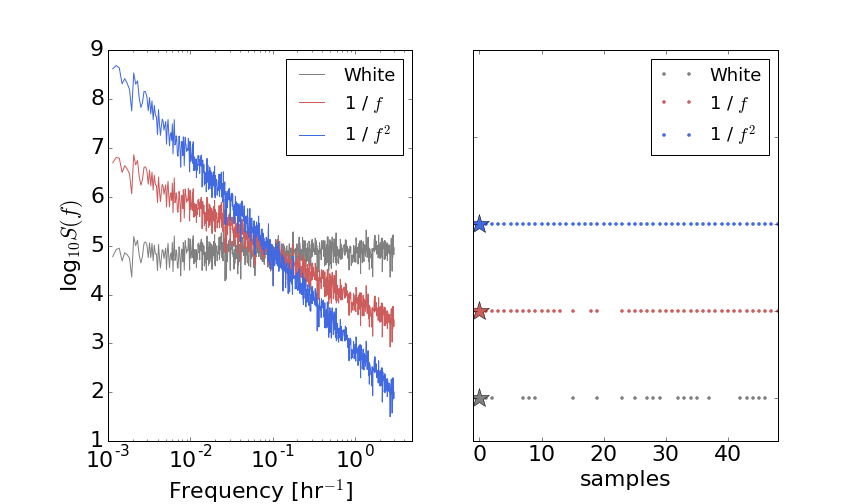
\includegraphics[trim={.5in, 0in, .5in, 0in}, width=0.5\textwidth, height=0.27\textwidth]{frb_sim_pink24.png}
   \caption{Realization of our mock follow-up Monte Carlo. \textit{Left panel}: Power spectrum for pulse arrival times of a single FRB.
   Grey shows a flat spectrum, corresponding to the often assumed Poissonian 
   repetition rate. The red and blue spectra show flicker noise, with pink (1/$f$) 
   noise and Brownian (1/$f^2$) noise respectively. \textit{Right panel}: 
   We found the first ``event" in our Monte Carlo (represented by a star) for the three different spectra 
   and plotted their behaviour in the subsequent 48 hours of followup. Though the average
   probability over the whole simulation is 0.5 for each distribution, when we zoom in 
   on this short period the strong time-like correlations 
   in the $1/f^\gamma$ cases means there are many repetitions: they are in an ``on" state at this time.}
   \label{FIG-RATE}
\end{figure}


\subsection{FRBs 110220 and 140514}
Using the event rate of $\sim10^4$ sky$^{-1}$ day$^{-1}$
from \cite{2013Sci...341...53T}, it 
was originally reported that the probability of seeing a 
new FRB in the field of 110220 during the 85 hours of follow-up 
was $\sim$0.32  
\citep{2015MNRAS.447..246P}. It was then pointed out by \cite{2015arXiv150701002M} 
that this underestimated the coincidence by an order of magnitude, 
since they estimated the rate in any one of the 13 beams, 
while the new event occurred in the identical beam.
The probability also dropped due to the updated daily event rate,
given the \cite{2013Sci...341...53T} estimate is now likely thought to be high.
In general we expect the true rate of FRBs to be lower than what is 
reported due to non-publication bias: If archival data is searched and 
nothing is found, it is less likely to be published than if something is found. 
That said, using the rate calculated in \cite{2015arXiv150500834R} and following
the procedure of \cite{2015arXiv150701002M}, we find the likelihood of 
$\sim$ 0.25-2.5$\%$.

Given the relatively low probability of finding 
a new FRB in the same field and since there are models that predict
burst repetition with variable DMs \citep{2015arXiv150505535C, 2015arXiv150701002M}
one can ask the question: If one FRB out of eight is found to
repeat during 110 hours of follow-up (including extra time spent on 140514), 
what are the limits on the expected
repeat period? Another way of asking this question is what is the probability of 
a some number of repetitions during the 110 hours, given a repeat rate. The answer to 
this question depends strongly on the powerspectrum's shape. For the sake of example, if the average 
repeat rate is once per hour, then the probability of one repeat or fewer in the Poisson
cats is effectively zero. With a pink distribution it is closer to $1\%$. 


\begin{figure}
  \centering
   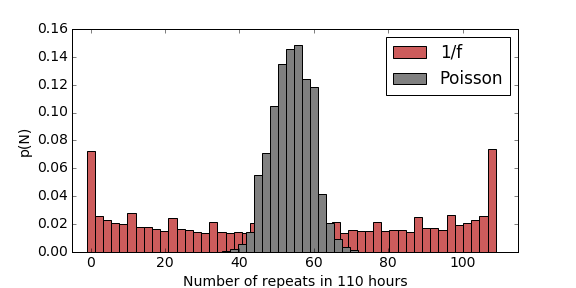
\includegraphics[trim={0in, 0in, 0in, 0in}, width=0.4\textwidth, height=0.23\textwidth]{110_hours_followup.png}
   \caption{Histogram of a 110-hours mock follow-up observation assuming an average repeat rate of 
   once per hour, using two different models 
   for the repetition statistics. The $y$-axis gives the probability density for seeing 
   N repetitions during the 110-hours observation.
   A 1$/f$ distribution (red) gives $\sim1\%$ probability of seeing one or zero events 
   (the two options, depending on the treatment of FRB 140514), 
   which is nearly impossible in the Poisson case (grey).}
   \label{FIG-hist}
\end{figure}


\section{Event rates and total number of sources}
\label{rate}

If FRBs were found to repeat, their statistics and the
average frequency of their repetition 
should affect the search strategy of upcoming surveys. 
For instance, if it were found that FRBs repeated,
on average, five times a day, then the number of unique 
sources would be five times smaller than the per-sky 
daily event rate. This means the rate 
$3.3^{+5.0}_{-2.5}\times10^3$ sky$^{-1}$ estimated by 
\cite{2015arXiv150500834R} would be produced by
only $\sim$160-1600 sources. In this scenario 
there is no FRB in most pixels on the sky, which means
one could integrate on most patches forever without 
seeing an event. An example of this strategy is the VLA millisecond search, 
in which $\sim40\%$ of the time was spent at a single pointing, and
almost three quarters of the time was spent at just three locations \citep{2015ApJ...807...16L}.
It is possible that pointing-to-pointing event rate variance contributed 
to their not seeing anything.

We therefore warn that deep surveys are at a disadvantage 
to those that sweep large regions of the sky 
(CHIME  \citep{2014SPIE.9145E..22B}, 
UTMOST\footnote{http://www.caastro.org/news/2014-utmost}, HIRAX)
because the non-repeating 
scenario is unaffected; whereas shallow observations 
should not hurt the detection rate, no matter what their repetition. 
Ideally, a survey
needs only to spend a few dispersion delay times on each beam 
before moving on. 

\section{Latitudinal dependence}
\label{latitude}
There is now evidence that the FRB rate is nonuniform on the sky, 
with fewer detectible events at low Galactic latitudes \citep{2014ira..book.....B}.
However the statistical significance of this finding may be 
overestimated. In \cite{2014ApJ...789L..26P}
the authors compute the probability of the disparity between the number of 
bursts seen in the the high and intermediate latitude ($|b| < 15\degree$)
 components of the High Time Resolution Universe survey 
(HTRU). They calculate the probability of seeing N=0 in the low-lat survey and M=4 in 
the high-lat, despite having searched 88$\%$ more data in the latter, and they 
rule out the uniform sky hypothesis with 99.5$\%$ certainty. We would point out 
that in general P(N$|$M) describes a very specific outcome, and P($\le$N$|\ge$M) would be 
more appropriate since it includes all outcomes equally or more unlikely.
That number might also be multiplied by two, since if the survey found 
four low-latitude FRBs and zero high-lat ones, we would ask the same question. HTRU 
has since reported five more bursts in the high Galactic region, but using a dataset 
that spent $\sim$2.5 times more time at high-lat. Below we try and quantify the likelihood of 
this.


If one wants to 
compare two statistical hypotheses, then the claims of each should 
be treated as true and their likelihood discrepancy should be computed.
In the case of testing the abundance of FRBs at high latitudes,
the sky should be partitioned into high and low regions a priori 
(e.g. the predefined high-lat HTRU and its compliment). The rate in both regions 
is then taken to be the same, and the likelihood of a given spatial distribution of observed
sources can be calculated. This situation is naturally
described by a biased binomial distribution with a fixed number of events. Suppose
a total of K FRBs are observed in a given survey. We can ask the question, what is the probability of 
seeing M events in the high region and (K-M) events in the lower region? 
This probability can be calculated % Should I include >M in one region?
as 

\begin{equation}
\label{eq-binomial}
\textup{P(M} | \,\textup{K}, p) =  \binom{\textup{K}}{\textup{M}} \, p^{\textup{M}} (1-p)^{\textup{K}-\textup{M}} 
\end{equation}

\noindent where $p$ is the probability that an event happens to show up in the 
northern region. In a survey where more time is spent on one part of the 
sky than the other, $p=(1 + \alpha)/\, \alpha$, where $\alpha$ is the ratio of 
time spent in the high-lat region vs. the intermediate region. In the case of the HTRU 
survey, K=9 and since none were found 
in the low-lat region, M=9. Roughly 2500 hours were spent searching the upper region
and $\sim1000$ hours were spent at $|b| < 15\degree$, giving $\alpha=0.4$. Using equation 
\ref{eq-binomial}, this outcome is only $\sim5\%$ unlikely. 

The problem is given a quasi-Bayesian treatment in 
\cite{2014ApJ...789L..26P} which gives the following.

\begin{equation}
\label{eq-petroff}
\textup{P(N} | \,\textup{M}) =  \alpha^{\textup{N}} (1 + \alpha)^{-(1+\textup{M+N})} \frac{(\textup{M+N})!}{\textup{M!N!}}
\end{equation}

\noindent This gives a probability of $\sim$3.5$\%$. This method 
is Bayesian in the sense that they marginalize over the unknown rate 
and calculate a likelihood, but they then calculate a confidence 
and do not look at a posterior.  

However as mentioned 
above, If sticking with the Bayesian 
approach we should probably calculate

\begin{equation} 
\label{eq-petroff2}
\textup{P}(\le \textup{N}_{obs} | \ge \textup{M}_{obs}) = \sum_{0}^{N_{obs}} \sum_{M_{obs}}^\infty \textup{P(N} | \,\textup{M})
\end{equation} 

\noindent since we are concerned with the total likelihood of anything as or more 
extreme than the observed event. In the case where we do not see any in the low-lat 
region and N$_{obs}=0$, 

\begin{equation}
\textup{P}(\le \textup{N}_{obs} | \ge \textup{M}_{obs})=\frac{(1+\alpha)}{\alpha}^{-\textup{M}_{obs}}
\end{equation}

\noindent since equation \ref{eq-petroff2} becomes a geometric series sum. 
This gives a probability of $\sim$12$\%$, significantly larger than the non-integrated
calculation. 

The most obvious difference between the approach we have offered (biased coin-flip) 
and the quasi-Bayesian method is that we take M + N to be fixed. It follows to ask 
whether or not we \textit{should} regard the total number of FRBs as ``given"? 
We believe the answer is yes, since this is one of the few quantities that we 
have actually measured, along with M and N. What we are really trying 
to infer is how much larger $\mu_{high}$ is than $\mu_{low}$, so these 
rates should not be marginalized over. We calculate $P(\mu_{high} \le \alpha \mu_{low} | N, M)$
and find it to be 99.5$\%$ if you assume flat priors on $\mu_{high}$ and $\mu_{low}$.

Though clearly this is not the final word on the the latitudinal distribution of FRBs, 
we find the biased binomial approach to be the 
most transparent and intuitive treatment, while we are in the regime of small number statistics. 
Like \cite{2015arXiv150500834R} we argue
that the jury is still out on the severity of the latitudinal 
dependence. With current data the preference for FRBs to 
be discovered outside of the plane seems consistent with
sky-temperature effects and increased scattering. 
Whether or not more sophisticated explanations 
(e.g \cite{2015MNRAS.451.3278M}) are required remains to be seen. 

\section{Conclusions}

The search for FRBs with multiple surveys that have disparate sensitivities, 
frequency coverage, and survey strategy has made it difficult even to 
estimate a daily sky rate (not to mention publication bias). 
That combined with the relatively low number of total FRBs observed 
has meant that dealing with their statistics can be non-trivial. In 
the case of repetition, we remind the reader that several non-cataclysmic 
models for FRBs are expected to repeat. In the case of supergiant 
pulses from pulsars, SGR radio flares, or even Galactic flare stars, it is possible 
that this repetition would by non-stationary and might exhibit strong correlations 
in time. We have shown that if the repetition had some associated flicker noise 
and its powerspectrum were 1/$f^\gamma$, then one should expect the repetition 
rate to be higher immediately after the initial FRB detection. Therefore follow-up 
observations to archival discoveries that take place years or 
months after the first event would not provide strong upper limits. 
This also means that if no burst is found in a given beam after some 
integration time, then it is unlikely that one will occur in the following integration, and therefore 
a new pointing should be searched. In other words, shallow fast surveys are favourable. 

In section \ref{latitude} we offered a simple way of quantifying the 
latitudinal dependence of FRBs with a binomial distribution. This 
is akin to a biased coin flip, in which we ask ``what is the probability of 
M bursts being found in one region and N bursts in its compliment, given 
$\alpha$ times more time was spent in the latter". 

\section{Acknowledgements}


\newcommand{\araa}{ARA\&A}   % Annual Review of Astronomy and Astrophys.
\newcommand{\afz}{Afz}       % Astrofizica
\newcommand{\aj}{AJ}         % Astronomical Journal
\newcommand{\azh}{AZh}       % Astronomicekij Zhurnal
\newcommand{\aaa}{A\&A}      % Astronomy and Astrophysics
\newcommand{\aas}{A\&AS}     % Astronomy and Astrophys. Supplement Series
\newcommand{\aar}{A\&AR}     % Astronomy and Astrophysics Review
\newcommand{\apj}{ApJ}       % Astrophysical Journal
\newcommand{\apjs}{ApJS}     % Astrophysical Journal Supplement Series
\newcommand{\apjl}{ApJ}      % Astrophysical Journal Letters
\newcommand{\apss}{Ap\&SS}   % Astrophysics and Space Science
\newcommand{\baas}{BAAS}     % Bulletin of the American Astron. Society
\newcommand{\jaa}{JA\&A}     % Journal of Astronomy and Astrophysics
\newcommand{\mnras}{MNRAS}   % Monthly Notices of the Roy. Astron. Society
\newcommand{\nat}{Nat}       % Nature
\newcommand{\pasj}{PASJ}     % Publ. of the Astron. Society of Japan
\newcommand{\pasp}{PASP}     % Publ. of the Astron. Society of the Pacific
\newcommand{\paspc}{PASPC}   % Publ. Astron. Soc. Pacific Conf. Proc.
\newcommand{\qjras}{QJRAS}   % Quart. Journal of the Royal Astron. Society
\newcommand{\sci}{Sci}       % Science
\newcommand{\solphys}{Solar Physics}       % 
\newcommand{\sova}{SvA}      % Soviet Astronomy
\newcommand{\aap}{A\&A}
\newcommand\jcap{{J. Cosmology Astropart. Phys.}}%
\newcommand{\prd}{Phys. Rev. D}

%\bibliography{frb}
\bibliography{frb_statistics}
\bibliographystyle{mn2e}


\label{lastpage}


\end{document}


